\section{Motivating Example} \label{sec:motivating_example}

 \begin{figure*}[t]
	\centering 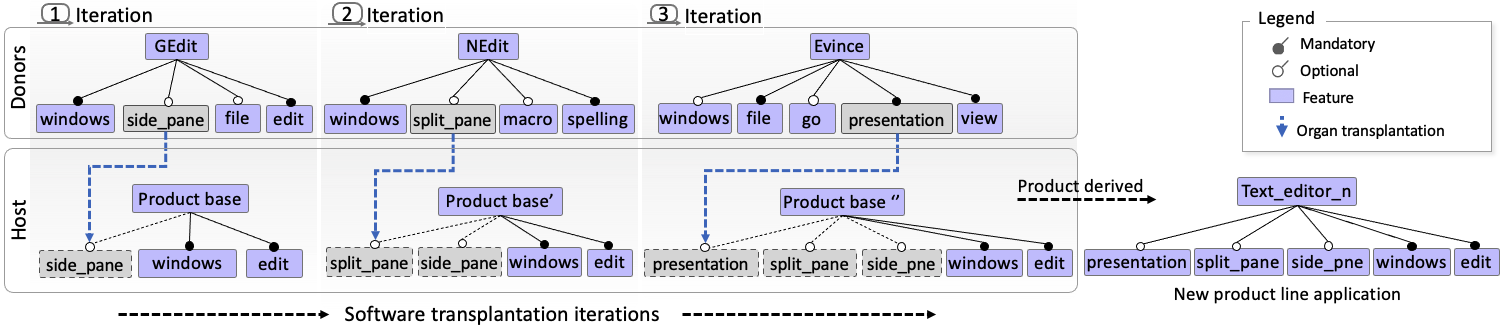
\includegraphics[width=\textwidth]{images/incremental_ST4.png}
	\caption{Product derivation process using the \FOUNDRY approach. \textit{\prodscalpel transplants three features, in sequence, into the GEdit's product base to derive a new text editor after three iterations of organ transplantation.} }
	\label{fig:incremental_pd}
\end{figure*} 
 %COMMENT: \ls{The case for SPL needs to be elaborated:  we must argue that the various GNOME subprojects share sufficient code to define a product base.  If too many of them are too different, SPL would be inappropriate.}
%\todo{This sentence is problematic:  we shoudl discuss. Done}
%\eb{from Leandro: I've rewritten this sentence by providing details of how GNOME could benefit from using SPLE principles as mass customisation and a common platform.}

The open-source GNOME project\footnote{https://wiki.gnome.org/Projects} encompasses a large portfolio of individual programs evolve as independently as possible from the rest. These programs share features, but because they are separately developed, their constituent features cannot be easily reused across its portfolio to provide mass customization, at least without much manual effort. The combination of mass customisation and a common platform, principles of Software Product Line Engineering (SPLE)~\cite{Pohl2005}, would allows to GNOME team reuses a common base of technology and, at the same time, to bring out products tailored individual customers. Without a common platform and a software development process base on mass customisation, it may be more difficult to the GNOME project provides customized products and effectively manage the commonality and variability of its features.

The GNOME  project is a natural candidate for SPL, but the significant reengineering investment of time and resources have prevented it from adopting SPL. \FOUNDRY is transformative because it can be used to reduce this cost. 

We show how the GNOME team could use \prodscalpel to quickly generate a product line. Suppose project collaborators want to build a product line in the domain of text editors. This product line would allow GNOME to produce text editors that augment its current text editor, \emph{GEdit}\footnote{https://wiki.gnome.org/Apps/Gedit}, with additional features. Since they have decided to augment Gedit, GNOME team would select it as the product base, the shared substrate of a product line that, for \FOUNDRY, serves the host for transplanted features.  Assume that the GNOME team targets the following three features (1) $\texttt{side-panel}$, (2) $\texttt{split pane}$, and (3) $\texttt{presentation}$. They then identify two donors from which to transplant these features:  \emph{NEdit}\footnote{https://sourceforge.net/projects/nedit/}, a multi-purpose text editor that is not part of the GNOME portfolio, and \emph{Evince}\footnote{https://wiki.gnome.org/Apps/Evince}, a document viewer for multiple document formats that is part of GNOME, not not an editor. 
 
\prodscalpel iteratively and incrementally re-engineers the codebase for SPL.  In the donor, engineers need to demarcate all feature entry points to transplant; a single annotation is sufficient for \prodscalpel to extract a feature. 
%\todo{remove: To prepare the host, GNOME engineers use \prodscalpel to extract a product base by removing all not desired features. }

To prepare the host, GNOME engineers use \prodscalpel to extract a product base from an existing system by removing all features not shared across all products within the built product line
 
Then, the engineers must annotate the host to indicate the implantation point for each target feature, or “organ” using transplantation nomenclature. GNOME engineers then run \prodscalpel on these inputs, once per feature, with 
%\ls{This listing is better.  First, the important thing is to show what a user would \emph{actually} type!  Doing so subtly shows that the system is real.  This text is nothing real and, as such, it invalidates the sentence that proceeds it.  Second, why define these switches?  They're self-defining!  What could the switch "donor\_folder" mean other that the path to the donor source code? I am leaving this todo here briefly for you to read it before I revert your change.  I'm trying to avoid churn.  I would like your help with which ones you think are mandatory.  Many should be either defaulted or in a configuration file, not on the command line.  Thinking more about that, maybe all are configuration, not CLI, and we should present a config file here with a minimal CLI invocation.} \eb{I'm with you Earl, all parameters of this command can be considered configuration. I can improve it in the next version of the ProducScalpel or during the journal review process. Do you prefer I remove this command for the moment?}
\begin{quote}
    $\texttt{./prodScalpel \textemdash \textemdash seeds\_file}$: \textit{ The file which contains the seeds for Genetic Programming(GP) algorithm.} 

    $\texttt{\textemdash \textemdash donor\_folder}$: \textit{The path to the donor source code.} 
    
    $\texttt{\textemdash \textemdash host\_target}$: \textit{The file in host that contains the insertion point of the transplant.}
    
    $\texttt{\textemdash \textemdash donor\_target}$: \textit{The file in the donor that contains the core function.}
    
    $\texttt{\textemdash \textemdash workspace}$: \textit{The path to the workspace of the transplant.}
    
    $\texttt{\textemdash \textemdash core\_function\_target}$: \textit{The file which contains all feature entry points.}
    
     $\texttt{\textemdash \textemdash  host\_project}$: \textit{The path to the product base source code.}
     
   \end{quote} 
%
%\begin{lstlisting}[language=bash]
%prodScalpel --seeds_file <transplantation_directory>/seed-1.in 
%    --compiler_options <transplantation_directory>/CFLAGS
%    --host_target <transplantation_directory>/productBase/insert_point_file.c 
%    --donor_target <donor_directory>/Donor/organ_souce_file.c 
%    --donor_folder <donor_directory>/Donor/
%    --workspace <transplantation_directory>/ 
%    --core_function <core_funtion_name> 
%    --host_project <transplantation_directory>/ProductBase
%\end{lstlisting}
%
%\ls{\lstinline+<root>+ is used without definition.  How can the Donor and Host share the same root?  That undercuts our contribution that the Donor can be unaware of the host!  Some of these switches look like they can be defaults, like seeds and compiler\_options and NOT reported/shown here.}

This command automatically extracts all of the specified feature's source code and its dependencies, or “over-organ” using transplantation nomenclature. More operational parameters are available at the project: webpage~\cite{ProjectWebpage}.

\Cref{fig:incremental_pd} illustrates all transplantation iterations performed to generate a new product.  It shows a new text editor derived from the transplant of features from different donors and using GEdit as a product base. Using feature models~\cite{Kang1990} to represent each donor system and the product base evolution, \prodscalpel first transplants the \emph{side-panel} feature, extracted from GEdit itself. This transplantation demonstrates that \prodscalpel can transplant features into a product base that comes from the same codebase.  Next, \prodscalpel transplants the \emph{split\_pane} feature from NEdit. It shows how \prodscalpel manages to transplant features from distinct codebases, which is not possible without manual effort using the current state-of-art to SPL reengineering. Finally, \prodscalpel transplants the \emph{presentation} feature from GNOME's Evince renderer. 

\FOUNDRY facilitates transplanting features from any program into a product line, opening the door to large scale feature reuse. Open-source projects, like GNOME, are an especially promising source of code for \FOUNDRY, so long as the donors and target hosts share compatible licenses.

